\documentclass[aspectratio=169]{../latex_main/tntbeamer}  % you can pass all options of the beamer class, e.g., 'handout' or 'aspectratio=43'
\usepackage{dsfont}
\usepackage{bm}
\usepackage[english]{babel}
\usepackage[T1]{fontenc}
%\usepackage[utf8]{inputenc}
\usepackage{graphicx}
\graphicspath{ {./figures/} }
\usepackage{algorithm}
\usepackage[ruled,vlined,algo2e,linesnumbered]{algorithm2e}
\usepackage{hyperref}
\usepackage{booktabs}
\usepackage{mathtools}

\usepackage{amsmath,amssymb}

\DeclareMathOperator*{\argmax}{arg\,max}
\DeclareMathOperator*{\argmin}{arg\,min}

\usepackage{amsbsy}
\newcommand{\vect}[1]{\bm{#1}}
%\newcommand{\vect}[1]{\boldsymbol{#1}}

\usepackage{pgfplots}
\pgfplotsset{compat=1.16}
\usepackage{tikz}
\usetikzlibrary{trees} 
\usetikzlibrary{shapes.geometric}
\usetikzlibrary{positioning,shapes,shadows,arrows,calc,mindmap}
\usetikzlibrary{positioning,fadings,through}
\usetikzlibrary{decorations.pathreplacing}
\usetikzlibrary{intersections}
\pgfdeclarelayer{background}
\pgfdeclarelayer{foreground}
\pgfsetlayers{background,main,foreground}
\tikzstyle{activity}=[rectangle, draw=black, rounded corners, text centered, text width=8em]
\tikzstyle{data}=[rectangle, draw=black, text centered, text width=8em]
\tikzstyle{myarrow}=[->, thick, draw=black]

% Define the layers to draw the diagram
\pgfdeclarelayer{background}
\pgfdeclarelayer{foreground}
\pgfsetlayers{background,main,foreground}

% Requires XeLaTeX or LuaLaTeX
%\usepackage{unicode-math}

\usepackage{fontspec}
%\setsansfont{Arial}
\setsansfont{RotisSansSerifStd}[ 
Path=../latex_main/fonts/,
Extension = .otf,
UprightFont = *-Regular,  % or *-Light
BoldFont = *-ExtraBold,  % or *-Bold
ItalicFont = *-Italic
]
\setmonofont{Cascadia Mono}[
Scale=0.8
]

\renewcommand{\ttdefault}{Cascadia Mono}

% scale factor adapted; mathrm font added (Benjamin Spitschan @TNT, 2021-06-01)
%\setmathfont[Scale=1.05]{Libertinus Math}
%\setmathrm[Scale=1.05]{Libertinus Math}

% other available math fonts are (not exhaustive)
% Latin Modern Math
% XITS Math
% Libertinus Math
% Asana Math
% Fira Math
% TeX Gyre Pagella Math
% TeX Gyre Bonum Math
% TeX Gyre Schola Math
% TeX Gyre Termes Math

% Literature References
\newcommand{\lit}[2]{\href{#2}{\footnotesize\color{black!60}[#1]}}

%%% Beamer Customization
%----------------------------------------------------------------------
% (Don't) Show sections in frame header. Options: 'sections', 'sections light', empty
\setbeamertemplate{headline}{empty}

% Add header logo for normal frames
\setheaderimage{
	% 
\includegraphics[height=\logoheight]{figures/TNT_darkv4.pdf}
	
\includegraphics[height=\logoheight]{../latex_main/figures/Leibniz-AI-Academy_Logo}
	% 
\includegraphics[height=\logoheight]{figures/logo_tntluh.pdf}
}

% Header logo for title page
\settitleheaderimage{
	% 
\includegraphics[height=\logoheight]{figures/TNT_darkv4.pdf}
	
\includegraphics[height=\logoheight]{../latex_main/figures/Leibniz-AI-Academy_Logo}
	% 
\includegraphics[height=\logoheight]{figures/logo_tntluh.pdf}
}

% Title page: tntdefault 
\setbeamertemplate{title page}[tntdefault]  % or luhstyle
% Add optional title image here
%\addtitlepageimagedefault{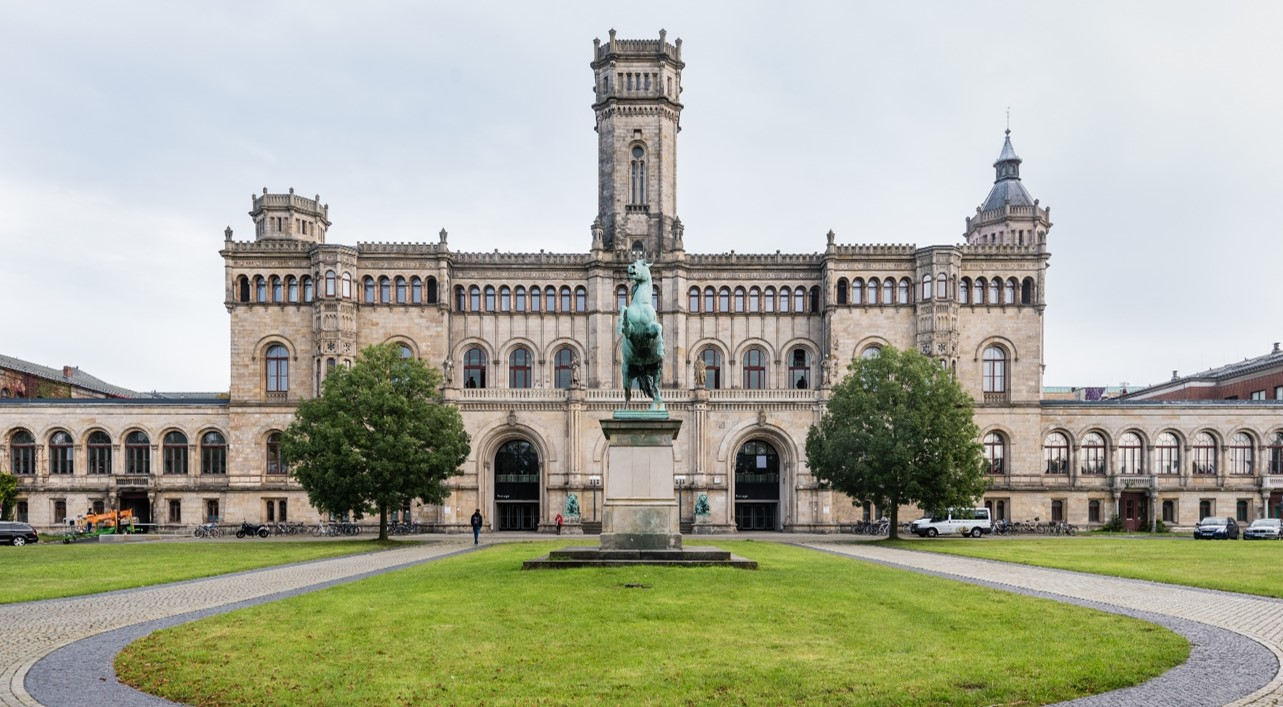
\includegraphics[width=0.65\textwidth]{figures/luh_default_presentation_title_image.jpg}}

% Title page: luhstyle
% \setbeamertemplate{title page}[luhstyle]
% % Add optional title image here
% \addtitlepageimage{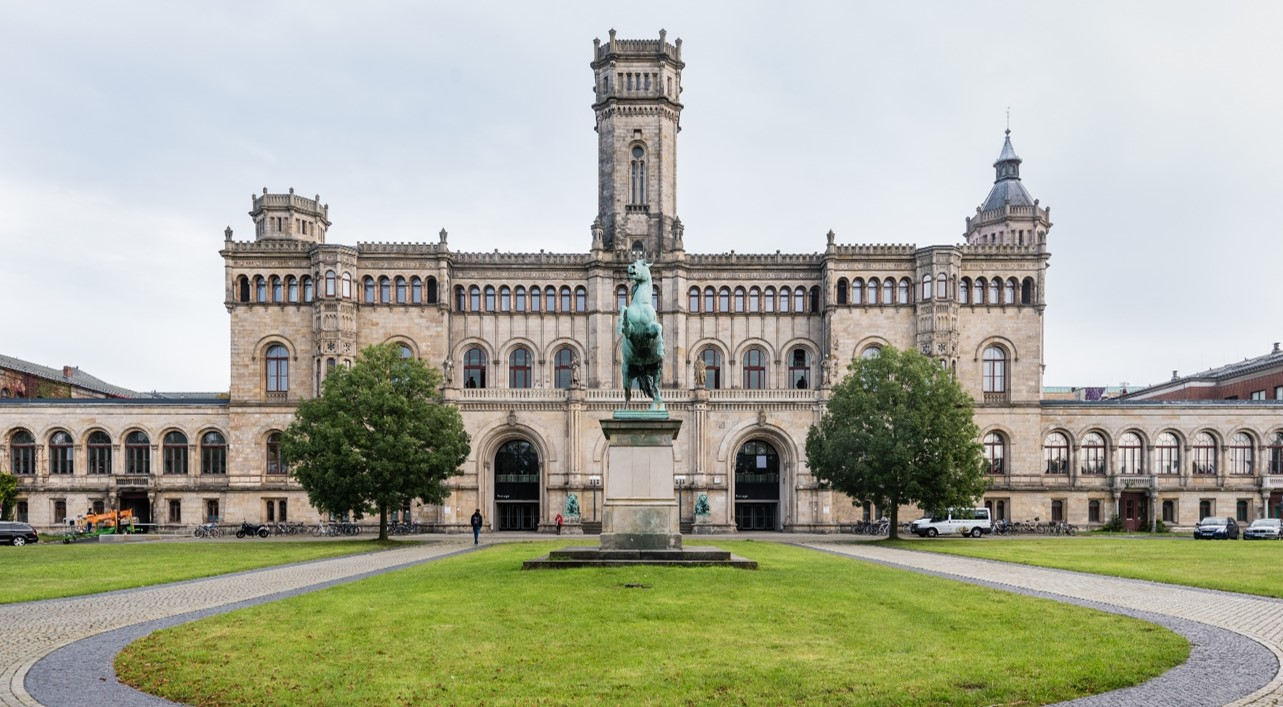
\includegraphics[width=0.75\textwidth]{figures/luh_default_presentation_title_image.jpg}}

\author[Abedjan \& Lindauer]{Ziawasch Abedjan \& \underline{Marius Lindauer}\\[1em]
	%
\includegraphics[height=\logoheight]{../latex_main/figures/luh_logo_rgb_0_80_155.pdf}\qquad
	
\includegraphics[height=\logoheight]{../latex_main/figures/DBIS_Kurzlogo.png}\qquad
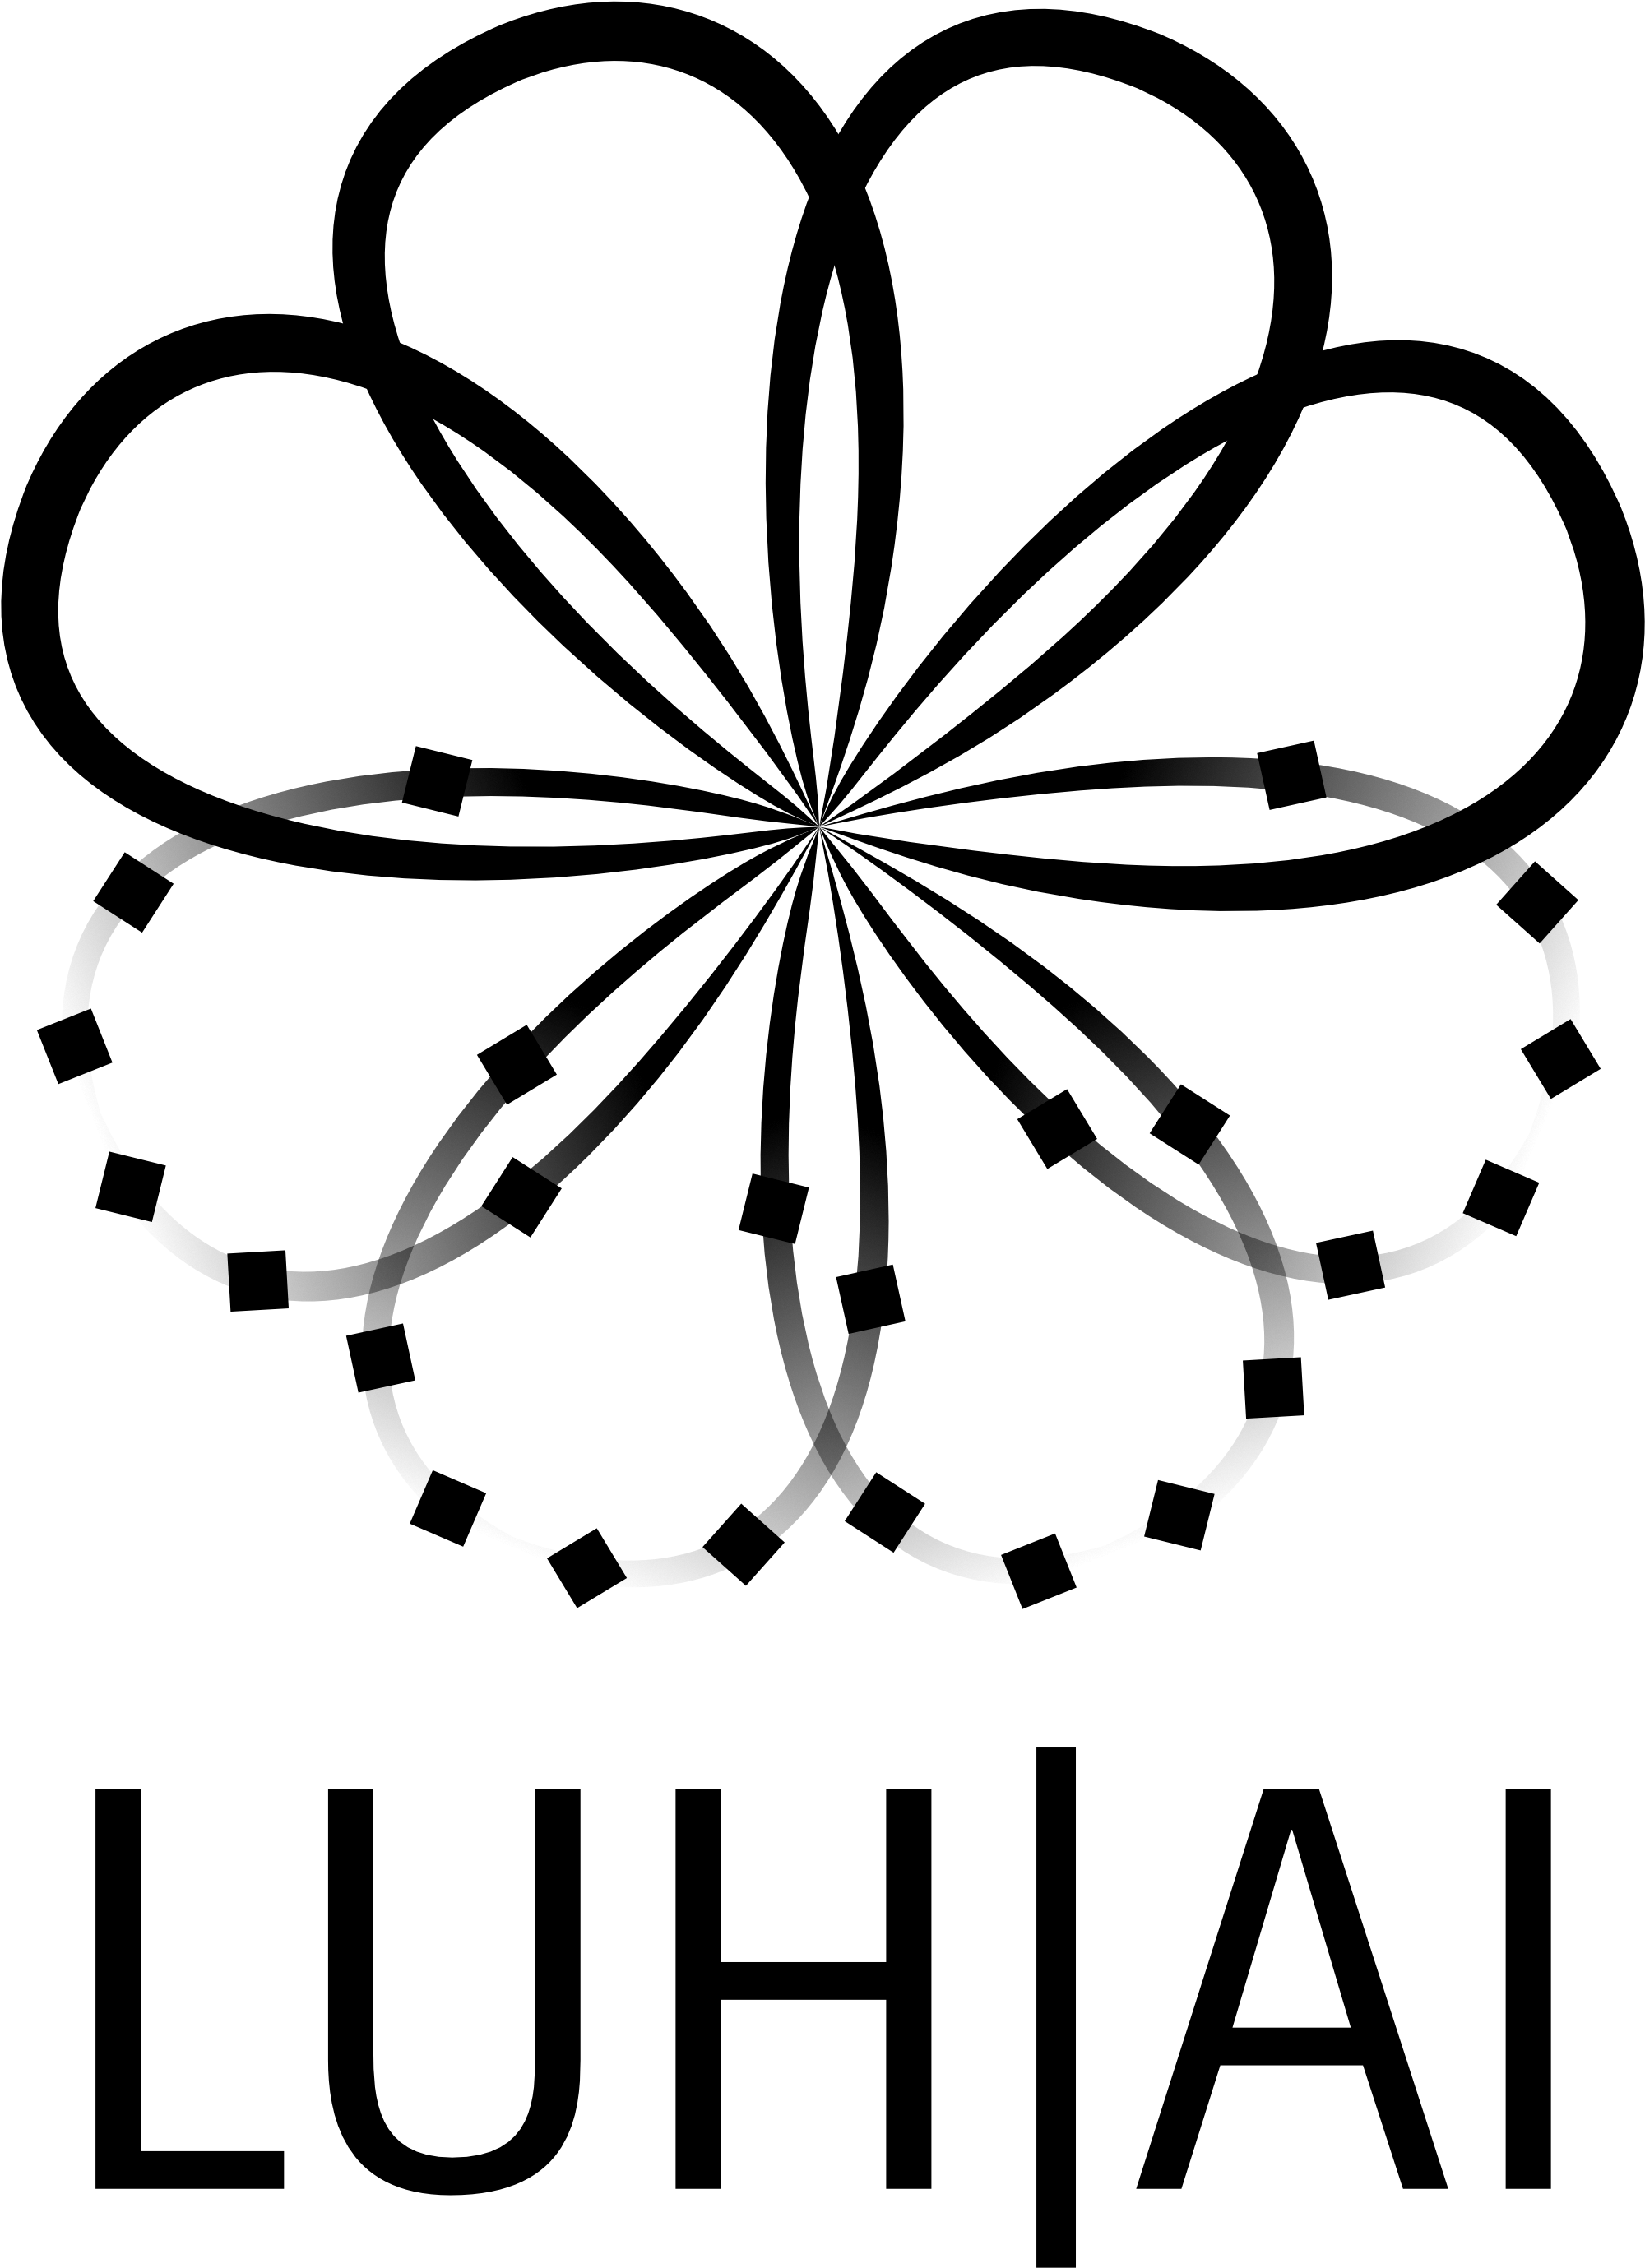
\includegraphics[height=\logoheight]{../latex_main/figures/logo_short_highres_black}\qquad

\includegraphics[height=\logoheight]{../latex_main/figures/Leibniz-AI-Academy_Logo}\qquad
%
\includegraphics[height=\logoheight]{../latex_main/figures/L3S.jpg}	
}
\date{\hspace{0.5em} {
\includegraphics[height=1.5em]{../latex_main/figures/Cc-by-nc-sa_icon.svg.png}}; extension of \href{https://ds100.org/fa21/}{[DS100]}
}


%%% Custom Packages
%----------------------------------------------------------------------
% Create dummy content
\usepackage{blindtext}

% Adds a frame with the current page layout. Just call \layout inside of a frame.
\usepackage{layout}


%%% Macros
%\renewcommand{\vec}[1]{\mathbf{#1}}
% \usepackage{bm}
%\let\vecb\bm

\title[Missing Values]{DS: Data Cleaning}
\subtitle{Missing Values}

\graphicspath{ {./figure/} }
%\institute{}

\date{\hspace{0.5em}{
\includegraphics[height=1.5em]{../latex_main/figures/Cc-by-nc-sa_icon.svg.png}}; extension of DS100 and Ziawasch Abedjan}

\begin{document}
	
	\maketitle
 
\begin{frame}
\frametitle{What to do with the Missing Values?}

\begin{itemize}
    \item Drop records with missing values
    \begin{itemize}
        \item Probably most common
        \item \textbf{Caution}: Check for biases introduced by dropped values
    \end{itemize}
    \item Missing or corrupt records might be related to something of interest
    \item Imputation: (Inferring missing values)
    \begin{itemize}
        \item \textbf{Mean Imputation}: Replace with an average value
        \begin{itemize}
            \item Which mean? Often use the closest related subgroup mean
        \end{itemize}
        \item \textbf{Hot deck imputation}: Replace with a random value
        \begin{itemize}
            \item Choose a random value from the subgroup and use it for the missing value
        \end{itemize}
        
    \end{itemize}
\end{itemize}

\end{frame}

\begin{frame}
\frametitle{Signs that your data may not be faithful}

\begin{itemize}
    \item \textbf{Missing Values} or default values
    \item \textbf{Truncated data} (e.g., early Excel limits: 65,536 Rows, 255 Columns)
    \begin{itemize}
        \item Solution: Be aware of consequences in analysis. How did truncation affect the sample?
    \end{itemize}
    \pause
    \item \textbf{Time Zone Inconsistencies}
    \begin{itemize}
        \item Solution 1: Convert to a common timezone (e.g., UTC)
        \item Solution 2: Convert to the timezone of the location – useful in modeling behavior
    \end{itemize}
    \pause
    \item \textbf{Duplicated Records or Fields}
    \begin{itemize}
        \item Solution: Identify and eliminate (use primary key); implications on sample?
    \end{itemize}
    \pause
    \item \textbf{Spelling Errors}
    \begin{itemize}
        \item Solution: Apply corrections or drop records not in a dictionary; implications on sample?
    \end{itemize}
    \pause
    \item \textbf{Units not specified or consistent}
    \begin{itemize}
        \item Solution: Infer units, check values are in reasonable ranges for data
    \end{itemize}
\end{itemize}

\end{frame}

\begin{frame}
\frametitle{(Disguised) Missing Values}

\centering
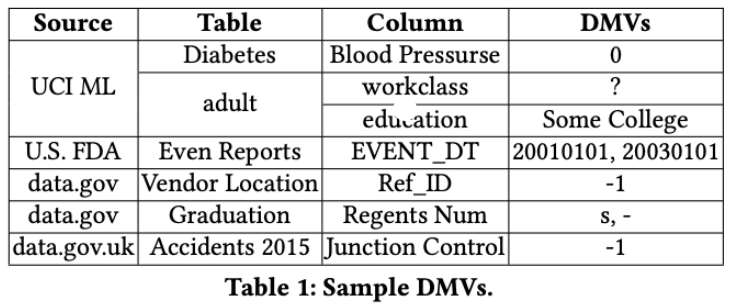
\includegraphics[width=0.8\textwidth]{figure/bild14_missing_values}

\begin{itemize}
    \item Refer to \url{https://dl.acm.org/doi/pdf/10.1145/3219819.3220109} for more details
\end{itemize}

\end{frame}

\begin{frame}
\frametitle{Classification of Errors}

\centering
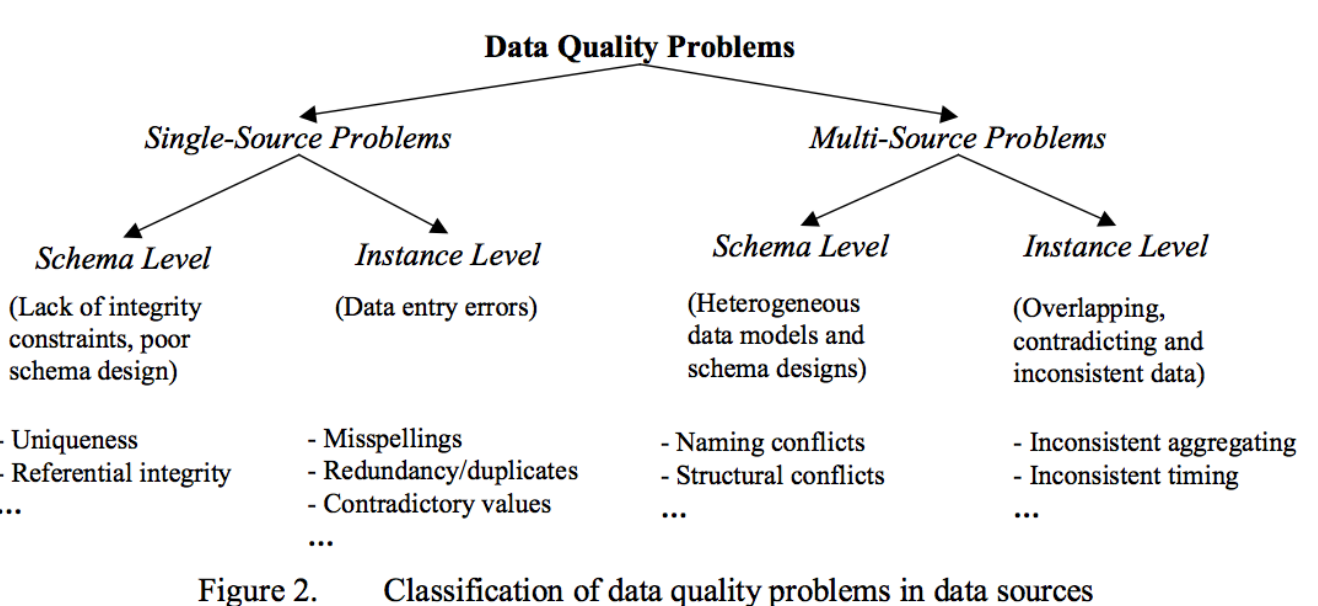
\includegraphics[width=0.8\textwidth]{figure/bild15_quality_problems.png}

\bigskip
\tiny
Erhard Rahm, Hong Hai Do: Data Cleaning: Problems and Current Approaches. IEEE Data Eng. Bull. 23(4): 3-13 (2000)

\end{frame}

\begin{frame}{Error Types}
    \begin{itemize}
        \item Based on the origin of the errors (e.g. spelling mistake) [Hellerstein 2008, Ilyas \& Chu 2015, Kim et al. 2003, Rahm \& Do 2000]
        \item General model: 
        \begin{itemize}
            \item Error = A value that is different from groundtruth
        \end{itemize}
        \item Based on discovery strategies:
    \end{itemize}

    \centering
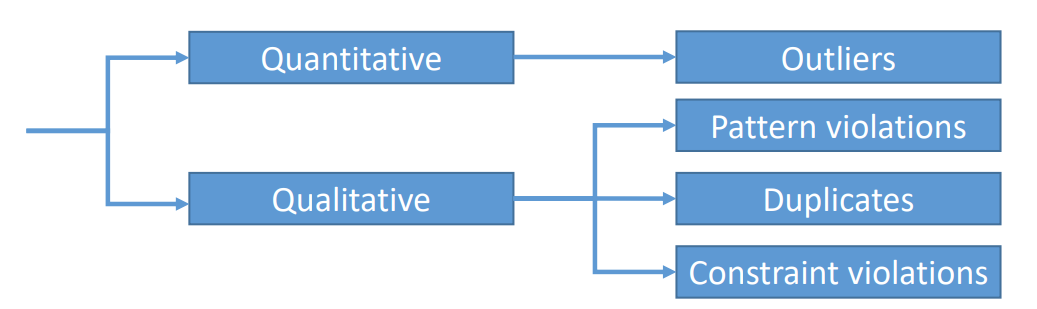
\includegraphics[width=0.8\textwidth]{figure/bild16_class_error.png}
    
\end{frame}

\begin{frame}
\frametitle{Error Detection Strategies}

\begin{enumerate}
    \item Rule-based detection algorithms
    \begin{itemize}
        \item Detecting violation of constraints, such as Zip Code $\rightarrow$ City
    \end{itemize}
    \item Pattern verification and enforcement tools
    \begin{itemize}
        \item Syntactical patterns, such as date formatting
        \item Semantical patterns, such as location names
    \end{itemize}
    \item Quantitative algorithms
    \begin{itemize}
        \item Statistical outliers
    \end{itemize}
    \item Deduplication
    \begin{itemize}
        \item Discovering conflicting attribute values in duplicates
    \end{itemize}
\end{enumerate}

\begin{itemize}
    \item \textbf{Examples:} 
    \begin{itemize}
        \item Salary = -1,000,000\$
        \item Date formats: mm/dd/yy vs. dd.mm.yyyy
        \item City name = “Peter Pane”, Zip = “10001” $\&$ City = “NYC”
    \end{itemize}
\end{itemize}

\end{frame}


\begin{frame}[c]{Aggregation of Error Detection Strategies [SSDBM’18]}

\begin{columns}

    \column{0.5\textwidth}
    
    \centering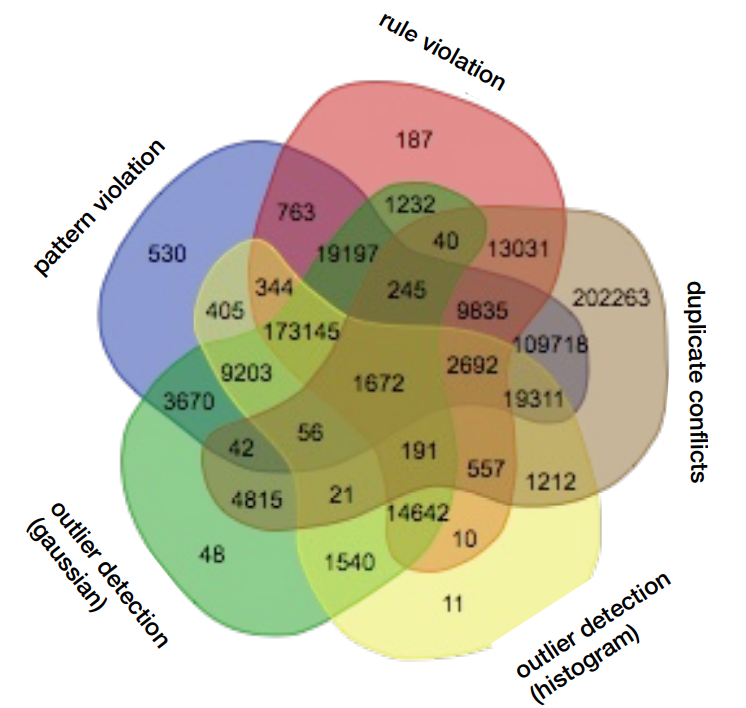
\includegraphics[width=0.9\textwidth]{figure/bild17_aggregation.png}


     \column{0.5\textwidth}

    \begin{itemize}
        \item Increasing number of systems in industry and academia [Claudel2016, Dallachiesa2013, Kandel2011]
        \item Data-Quality systems are tailored towards one data quality issue.
        \item Datasets often contain mixed issues (e.g., missing values and rule violations) [Arocena2015]
        %\item Previous work on heuristics-based aggregation: Union-All, Min-K, Precision-based Ordering [PVLDB'2016]
    \end{itemize}
    
\end{columns}


\end{frame}

\end{document}